\pgfplotsset{soldot/.style={color=blue,only marks,mark=*}} \pgfplotsset{holdot/.style={color=blue,fill=white,only marks,mark=*}}
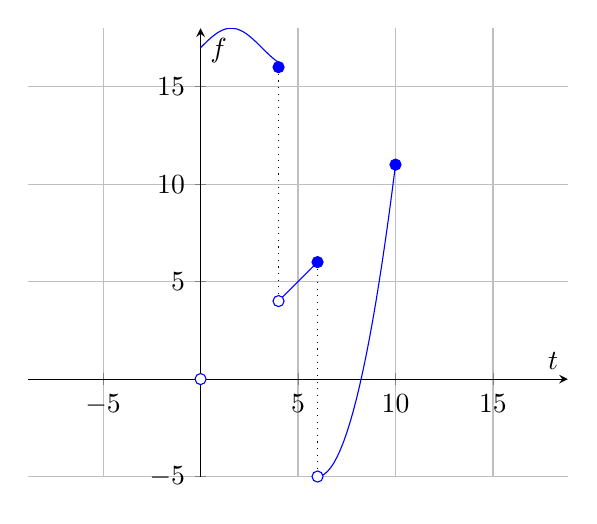
\begin{tikzpicture}
	\begin{axis}[axis lines=middle, axis equal, grid=both, xlabel = $t$, ylabel = $\operatorname{f}$]
		\addplot[domain=0:4, blue] {sin(deg(x)) + 17};
		\addplot[domain=4:6, blue] {x};
		\addplot[domain=6:10, blue] {(x - 6)^2 - 5};
		\draw[dotted] (axis cs:4,16) -- (axis cs:4,4);
		\draw[dotted] (axis cs:6,6) -- (axis cs:6,-5);
		\addplot[holdot] coordinates{(0,0)(4,4)(6,-5)};
		\addplot[soldot] coordinates{(4,16)(6,6)(10,11)};
	\end{axis}
\end{tikzpicture}